\documentclass[12pt]{article}


% -------------------- PAQUETES --------------------
\usepackage[utf8]{inputenc}
\usepackage[spanish]{babel}
\usepackage[margin=2.54cm]{geometry}
\usepackage{graphicx}
\usepackage{xcolor}


% -------------------- CARGA DE ARCHIVOS EXTERNOS --------------------
% ----------------- UTILIDADES PARA DAR UN MEJOR FORMATO DE DOCUMENTO -----------------  


\definecolor{azul}{rgb}{0.0039, 0.3098, 0.6196}


% Formato para el indice general ...........
\makeatletter
    \renewcommand{\@dotsep}{1.5}
    \renewcommand{\l@section}{\@dottedtocline{1}{1.5em}{2.3em}}
    \renewcommand{\l@subsection}{\@dottedtocline{2}{3.8em}{3.2em}}
    \renewcommand{\l@subsubsection}{\@dottedtocline{3}{7.0em}{4.1em}}
\makeatother

% --------- COMANDOS PERSONALIZADOS PARA LA PORTADA DE LAS TAREAS, TRABAJOS Y PROYECTOS ---------

\newcommand{\rutaLogo}[1]{\newcommand{\RutaLogo}{#1}}
\newcommand{\tema}[1]{\newcommand{\Tema}{#1}}
\newcommand{\etiquetaAutores}[1]{\newcommand{\EtiquetaAutores}{#1}}
\newcommand{\alumno}[1]{\newcommand{\Alumno}{#1}}
\newcommand{\materia}[1]{\newcommand{\Materia}{#1}}
\newcommand{\docente}[1]{\newcommand{\Docente}{#1}}
\newcommand{\ciclo}[1]{\newcommand{\Ciclo}{#1}}
\newcommand{\fecha}[1]{\newcommand{\Fecha}{#1}}
\newcommand{\periodo}[1]{\newcommand{\Periodo}{#1}}



% -------------------- DEFINICIÓN DE LA PORTADA --------------------
\rutaLogo{../../../../RecursosGlobales/Img/logo_tec_azuay.png}
\tema{\\ \vspace{1cm} Actividad N°3: Miscelánea de ejercicios de algoritmos de repetición \\ \vspace{1.7cm}}
\etiquetaAutores{Alumno:}
\alumno{Eduardo Mendieta \vspace{1cm}}
\materia{Introducción a la programación \vspace{1cm}}
\docente{Ing. Verónica Segarra \vspace{1cm}}
\ciclo{Primer Ciclo \vspace{1.1cm}}
\fecha{02 de julio de 2024 \vspace{1cm}}
\periodo{Abril 2024 - Agosto 2024}



% -------------------- INFORME --------------------
\begin{document}

    \begin{titlepage}

    \centering

    \includegraphics[width=0.11\textwidth]{\RutaLogo} 

    \vspace{0.3cm}
    \textcolor{azul}{\Large \textbf{Instituto Superior Universitario Tecnológico del Azuay \\}}
    \vspace{0.3cm}
    \textcolor{azul}{\Large \textbf{Tecnología Superior en Big Data}}
    
    % 1. ---------------- TEMA -------------------------
    
    {\Large\textbf{\Tema}}
    
    % 2. ---------------- AUTOR(ES) -------------------------
    \textcolor{azul}{\large \textbf{\EtiquetaAutores} \\}
    \vspace{0.3cm}
    {\large \Alumno}

    % 3. ---------------- MATERIA -------------------------
    \textcolor{azul}{\large \textbf{Materia:} \\}
    \vspace{0.3cm}
    {\large \Materia}


    % 3. ---------------- DOCENTE -------------------------
    \textcolor{azul}{\large \textbf{Docente:} \\}
    \vspace{0.3cm}
    {\large \Docente}


    % 3. ---------------- Ciclo -------------------------
    \textcolor{azul}{\large \textbf{Ciclo:} \\}
    \vspace{0.3cm}
    {\large \Ciclo}


    % 3. ---------------- FECHA -------------------------
    \textcolor{azul}{\large \textbf{Fecha:} \\}
    \vspace{0.3cm}
    {\large \Fecha}

    % 3. ---------------- PERIODO -------------------------
    \textcolor{azul}{\large \textbf{Periodo Académico:} \\}
    \vspace{0.3cm}
    {\large \Periodo}
 
\end{titlepage}

  
    \section*{\centering Actividad N°3}

        \textbf{Para los siguientes ejercicios, desarrollar: Diagrama de flujo, pruebas de escritorio y algoritmo en PseInt.}

        \begin{enumerate}
            % Ejercicio 1: -----------------------------------------------
            \item  Hacer un diagrama de flujo que imprima los números del 100 al 0, en orden decreciente.
            
                \begin{figure}[!h]
                    \centering
                    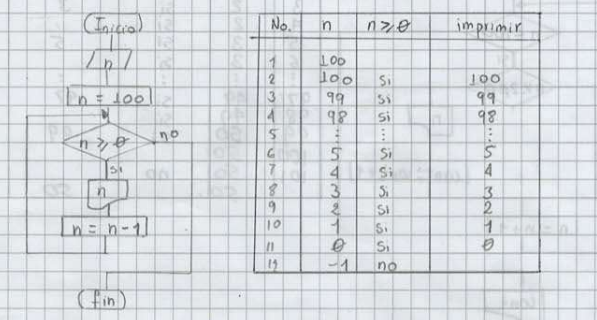
\includegraphics[width=0.9\textwidth]{Img/DF_ej1.png}
                \end{figure}

                
                \begin{figure}[!h]
                    \centering
                    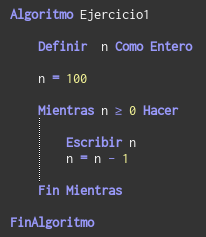
\includegraphics[width=0.3\textwidth]{Img/Cod_ej1.png}
                \end{figure}

                \newpage
                \begin{figure}[!h]
                    \centering
                    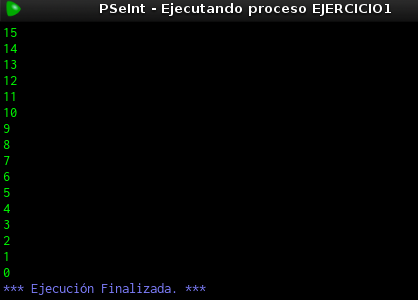
\includegraphics[width=0.6\textwidth]{Img/Ejec_ej1.png}
                \end{figure}

            % Ejercicio 2: -----------------------------------------------
            \newpage
            \item Hacer un diagrama de flujo que imprima los números pares entre 0 y 100.
            
                \begin{figure}[!h]
                    \centering
                    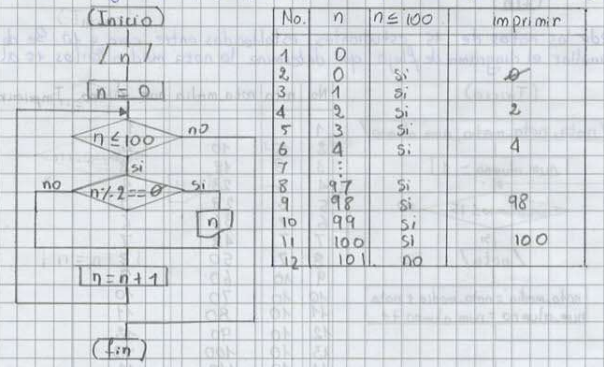
\includegraphics[width=0.9\textwidth]{Img/DF_ej2.png}
                \end{figure}

                \newpage
                \begin{figure}[!h]
                    \centering
                    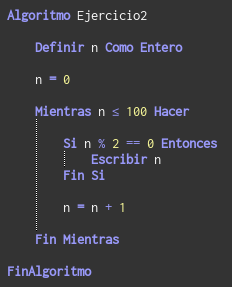
\includegraphics[width=0.5\textwidth]{Img/Cod_ej2.png}
                \end{figure}

                \begin{figure}[!h]
                    \centering
                    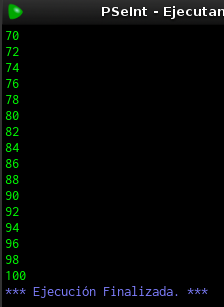
\includegraphics[width=0.4\textwidth]{Img/Ejec_ej2.png}
                \end{figure}

            % Ejercicio 3: -----------------------------------------------
            \newpage
            \item Hacer un diagrama de flujo que imprima los números impares hasta el 100 y que imprima cuantos impares hay.
            
                \begin{figure}[!h]
                    \centering
                    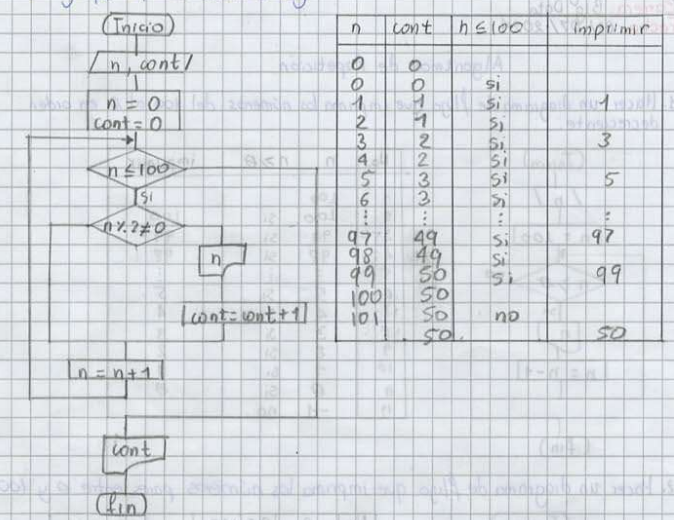
\includegraphics[width=0.9\textwidth]{Img/DF_ej3.png}
                \end{figure}

                \begin{figure}[!h]
                    \centering
                    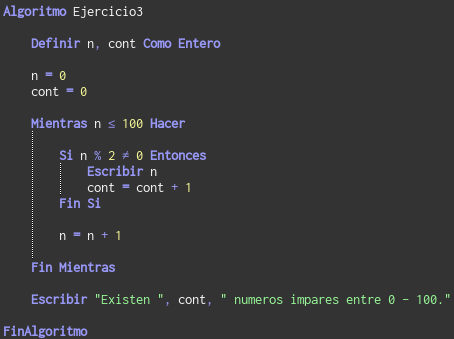
\includegraphics[width=0.7\textwidth]{Img/Cod_ej3.png}
                \end{figure}

                \begin{figure}[!h]
                    \centering
                    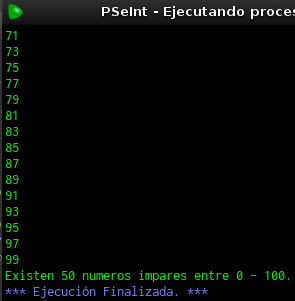
\includegraphics[width=0.5\textwidth]{Img/Ejec_ej3.png}
                \end{figure}
            
            % Ejercicio 4: -----------------------------------------------
            \newpage
            \item Pedir las notas de 15 estudiantes, establecidas entre cero y 10. Se desea desarrollar el diagrama de flujo que determine la nota media de los 15 alumnos.
            
                \begin{figure}[!h]
                    \centering
                    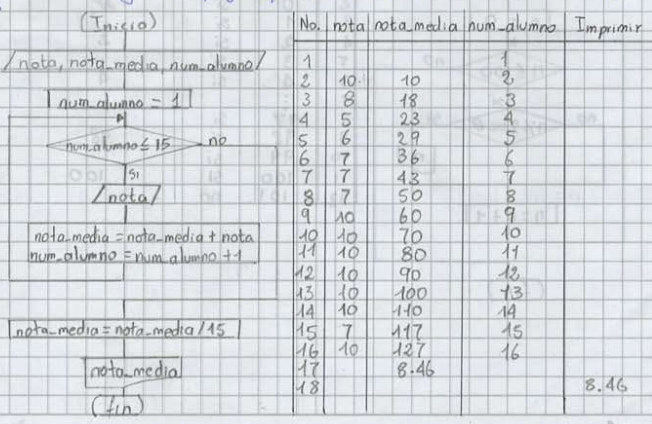
\includegraphics[width=0.8\textwidth]{Img/DF_ej4.png}
                \end{figure}

                \newpage
                \begin{figure}[!h]
                    \centering
                    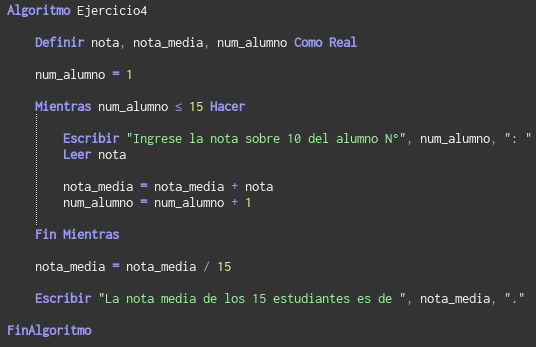
\includegraphics[width=0.6\textwidth]{Img/Cod_ej4.png}
                \end{figure}

                \begin{figure}[!h]
                    \centering
                    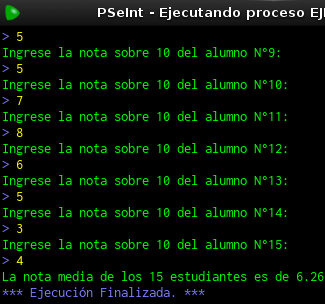
\includegraphics[width=0.6\textwidth]{Img/Ejec_ej4.png}
                \end{figure}

                
            % Ejercicio 5: -----------------------------------------------
            \newpage
            \item Ingresar un número, entero y efectuar la suma de todos los números que le anteceden, comenzando desde 0 y mostrar el resultado por pantalla.
            
                \begin{figure}[!h]
                    \centering
                    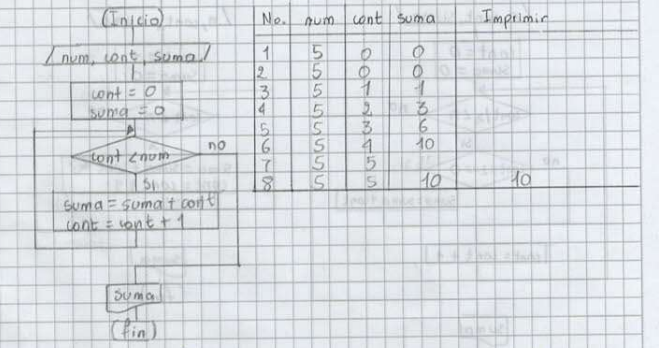
\includegraphics[width=0.9\textwidth]{Img/DF_ej5.png}
                \end{figure}

                \newpage
                \begin{figure}[!h]
                    \centering
                    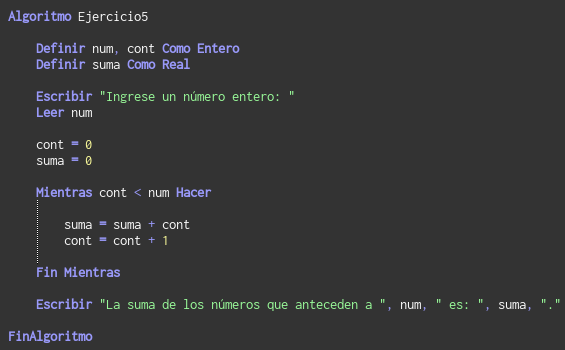
\includegraphics[width=0.9\textwidth]{Img/Cod_ej5.png}
                \end{figure}

                \begin{figure}[!h]
                    \centering
                    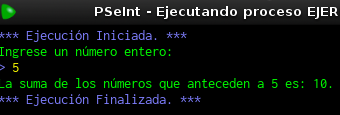
\includegraphics[width=0.7\textwidth]{Img/Ejec_ej5.png}
                \end{figure}
            
            % Ejercicio 6: -----------------------------------------------
            \newpage
            \item Hacer el diagrama de flujo para sumar los N primeros impares. Realizar después uno que haga lo mismo con los pares y, otro, con los múltiplos de 3.
                
                \begin{figure}[!h]
                    \centering
                    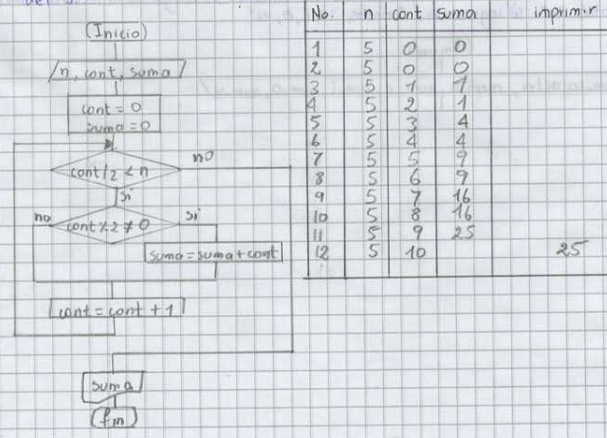
\includegraphics[width=0.7\textwidth]{Img/DF_ej6_1.png}
                \end{figure}

                \newpage
                \begin{figure}[!h]
                    \centering
                    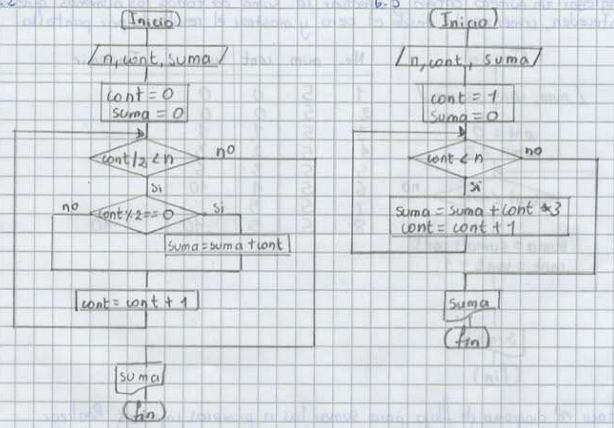
\includegraphics[width=0.9\textwidth]{Img/DF_ej6_2.png}
                \end{figure}

                \begin{figure}[!h]
                    \centering
                    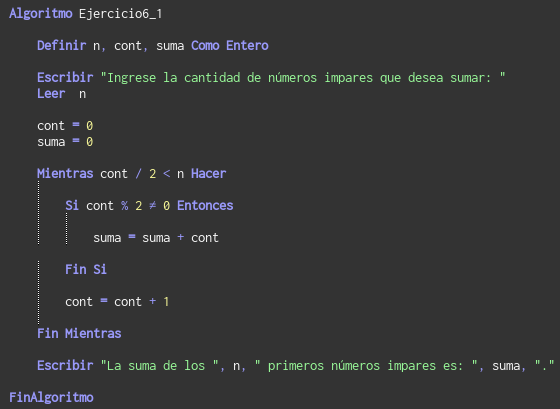
\includegraphics[width=0.8\textwidth]{Img/Cod_ej6_1.png}
                \end{figure}

                \begin{figure}[!h]
                    \centering
                    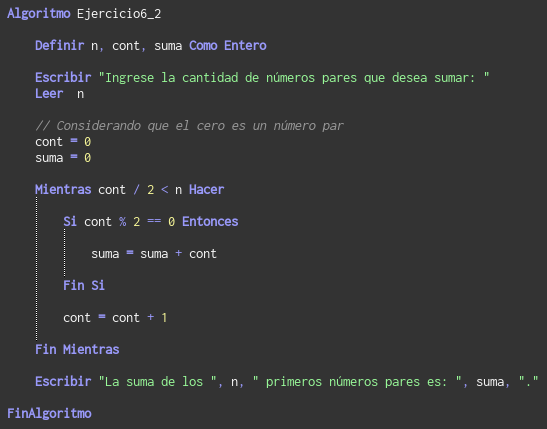
\includegraphics[width=0.8\textwidth]{Img/Cod_ej6_2.png}
                \end{figure}

                \begin{figure}[!h]
                    \centering
                    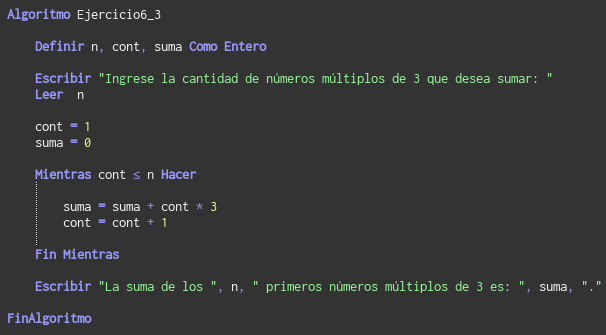
\includegraphics[width=0.8\textwidth]{Img/Cod_ej6_3.png}
                \end{figure}

                \begin{figure}[!h]
                    \centering
                    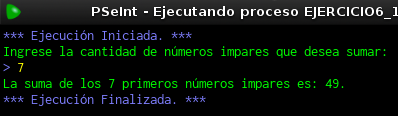
\includegraphics[width=0.7\textwidth]{Img/Ejec_ej6_1.png}
                \end{figure}

                \newpage
                \begin{figure}[!h]
                    \centering
                    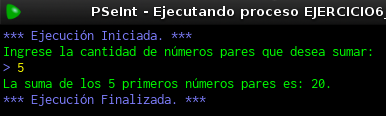
\includegraphics[width=0.7\textwidth]{Img/Ejec_ej6_2.png}
                \end{figure}

                \begin{figure}[!h]
                    \centering
                    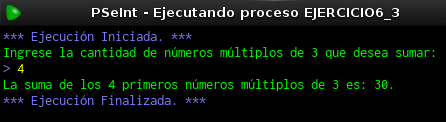
\includegraphics[width=0.7\textwidth]{Img/Ejec_ej6_3.png}
                \end{figure}
            
            % Ejercicio 7: -----------------------------------------------
            \newpage
            \item Escribir en Diagrama de flujo que lea 20 caracteres. Luego de la lectura indicar cuantas "a" se ingresaron, cuantas "e, i, o, u"

                \begin{figure}[!h]
                    \centering
                    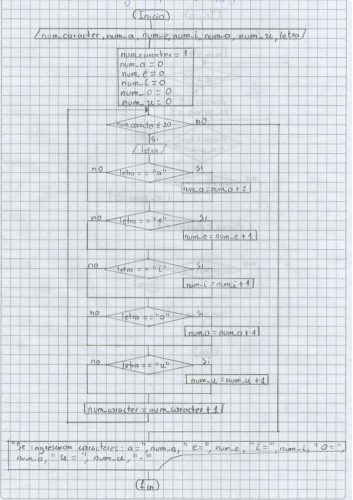
\includegraphics[width=0.9\textwidth]{Img/DF_ej7.png}
                \end{figure}

                \newpage
                \begin{figure}[!h]
                    \centering
                    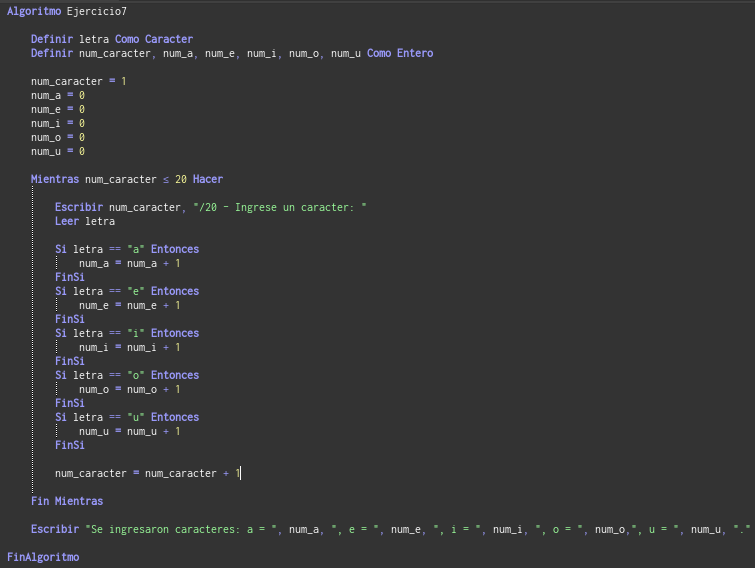
\includegraphics[width=0.8\textwidth]{Img/Cod_ej7.png}
                \end{figure}

                \begin{figure}[!h]
                    \centering
                    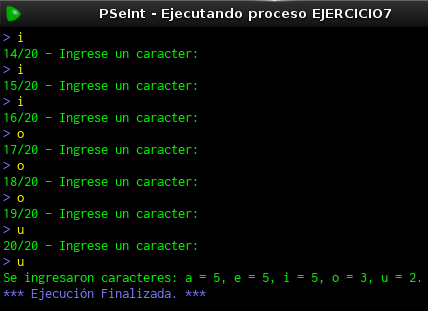
\includegraphics[width=0.8\textwidth]{Img/Ejec_ej7.png}
                \end{figure}

            
            % Ejercicio 8: -----------------------------------------------
            \newpage
            \item Escribir en Diagrama de flujo un algoritmo que muestre los números primos comprendidos entre 0 y 100.
           
                \begin{figure}[!h]
                    \centering
                    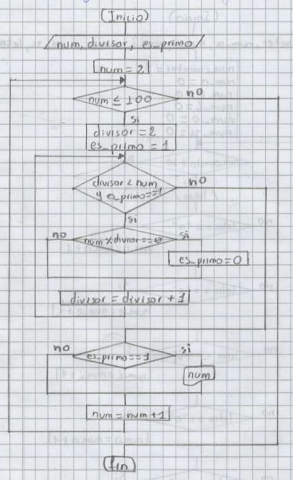
\includegraphics[width=0.6\textwidth]{Img/DF_ej8.png}
                \end{figure}

                \newpage
                \begin{figure}[!h]
                    \centering
                    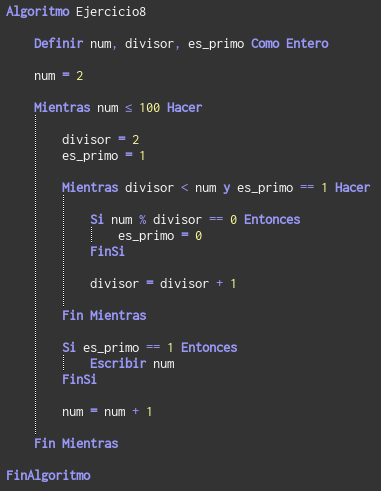
\includegraphics[width=0.6\textwidth]{Img/Cod_ej8.png}
                \end{figure}

                \newpage
                \begin{figure}[!h]
                    \centering
                    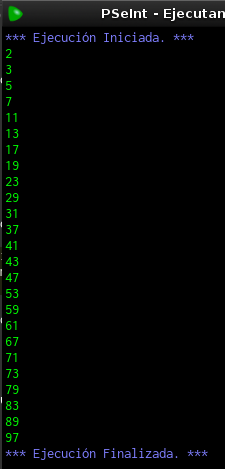
\includegraphics[width=0.3\textwidth]{Img/Ejec_ej8.png}
                \end{figure}
           
            % Ejercicio 9: -----------------------------------------------
            \newpage
            \item De 10 números ingresados indicar cuantos son mayores a cero y cuantos son menores a cero.
            
                \begin{figure}[!h]
                    \centering
                    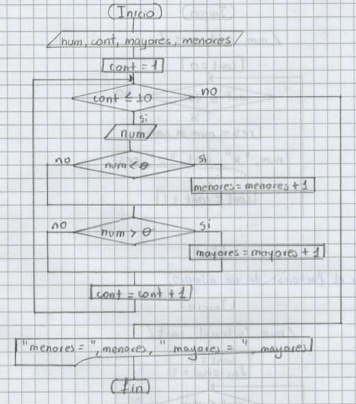
\includegraphics[width=0.6\textwidth]{Img/DF_ej9.png}
                \end{figure}

                \begin{figure}[!h]
                    \centering
                    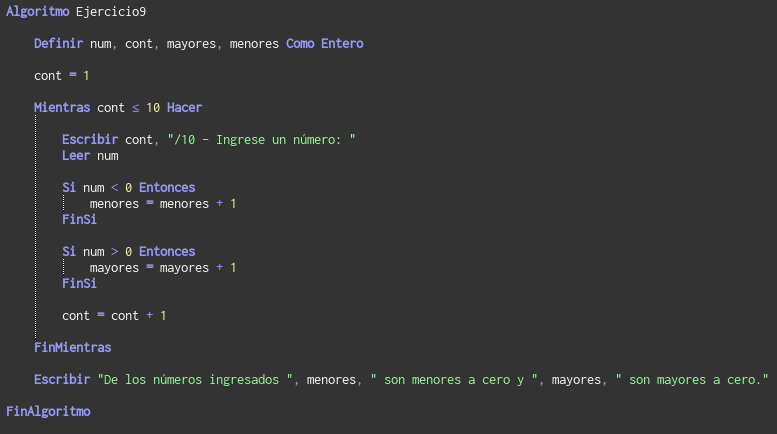
\includegraphics[width=0.8\textwidth]{Img/Cod_ej9.png}
                \end{figure}

                \newpage
                \begin{figure}[!h]
                    \centering
                    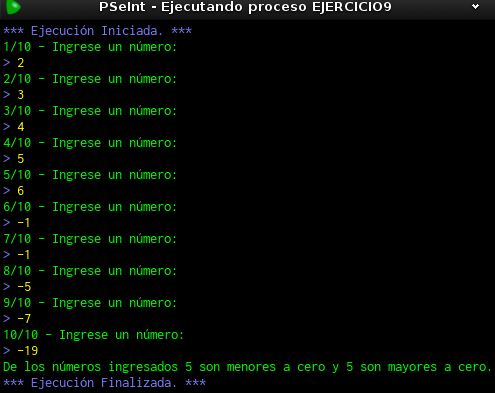
\includegraphics[width=0.5\textwidth]{Img/Ejec_ej9.png}
                \end{figure}
            
            % Ejercicio 10: -----------------------------------------------
            \newpage
            \item Realizar la tabla de multiplicar de un número entre 0 y 10 de forma que se visualice de la siguiente forma: 4x1=4 4x2=8.
        
                \begin{figure}[!h]
                    \centering
                    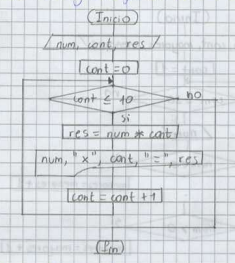
\includegraphics[width=0.6\textwidth]{Img/DF_ej10.png}
                \end{figure}

                \begin{figure}[!h]
                    \centering
                    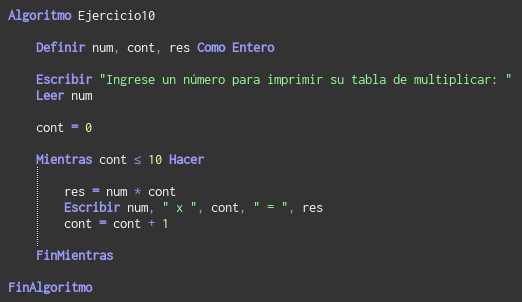
\includegraphics[width=0.6\textwidth]{Img/Cod_ej10.png}
                \end{figure}

                \begin{figure}[!h]
                    \centering
                    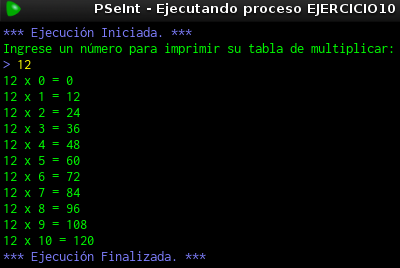
\includegraphics[width=0.5\textwidth]{Img/Ejec_ej10.png}
                \end{figure}

            % Ejercicio 11: -----------------------------------------------
            \newpage 
            \item Calcular la factorial de un número.
            
                \begin{figure}[!h]
                    \centering
                    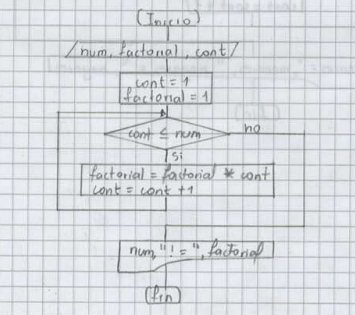
\includegraphics[width=0.6\textwidth]{Img/DF_ej11.png}
                \end{figure}

                \begin{figure}[!h]
                    \centering
                    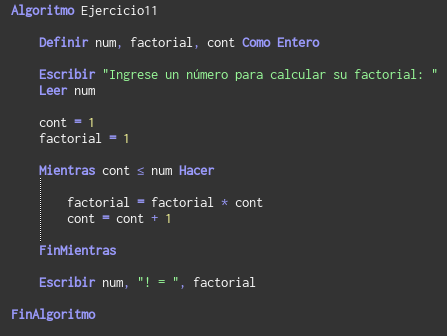
\includegraphics[width=0.6\textwidth]{Img/Cod_ej11.png}
                \end{figure}

                \begin{figure}[!h]
                    \centering
                    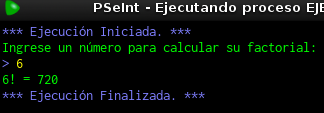
\includegraphics[width=0.5\textwidth]{Img/Ejec_ej11.png}
                \end{figure}
        
            % Ejercicio 12: -----------------------------------------------
            \newpage 
            \item Leer sucesivamente números del teclado hasta que aparezca un número comprendido entre 1 y 5.
                
                \begin{figure}[!h]
                    \centering
                    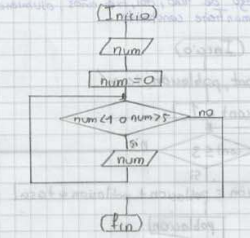
\includegraphics[width=0.6\textwidth]{Img/DF_ej12.png}
                \end{figure}

                \begin{figure}[!h]
                    \centering
                    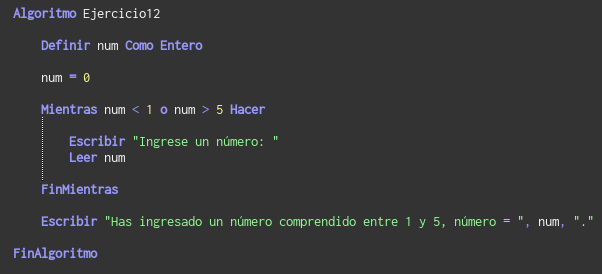
\includegraphics[width=0.6\textwidth]{Img/Cod_ej12.png}
                \end{figure}

                \begin{figure}[!h]
                    \centering
                    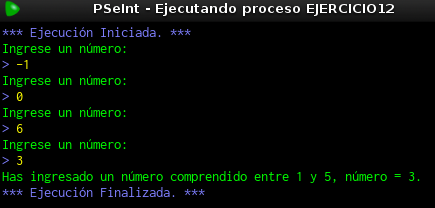
\includegraphics[width=0.5\textwidth]{Img/Ejec_ej12.png}
                \end{figure}

        
            % Ejercicio 13: -----------------------------------------------
            \newpage 
            \item Dados dos números enteros positivos N y D, se dice que D es un divisor de N si el resto de dividir N entre D es 0. Se dice que un número N es perfecto si la suma de sus divisores (excluido el propio N) es N. Por ejemplo 28 es perfecto, pues sus divisores (excluido elv28) son: 1, 2, 4, 7 y 14 y su suma es 1+2+4+7+14=28. Hacer un diagrama que dado un número N nos diga si es o no perfecto.
                
                \begin{figure}[!h]
                    \centering
                    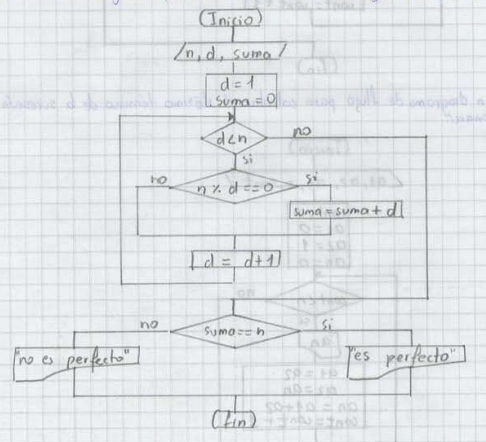
\includegraphics[width=0.6\textwidth]{Img/DF_ej13.png}
                \end{figure}

                \newpage
                \begin{figure}[!h]
                    \centering
                    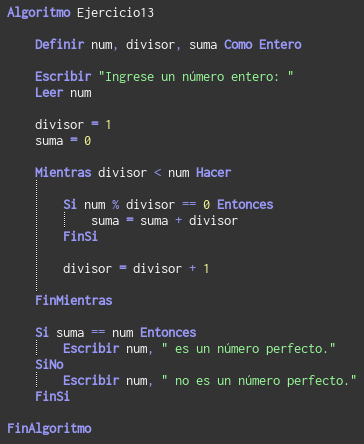
\includegraphics[width=0.6\textwidth]{Img/Cod_ej13.png}
                \end{figure}

                \begin{figure}[!h]
                    \centering
                    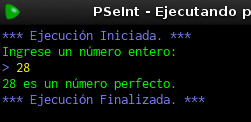
\includegraphics[width=0.5\textwidth]{Img/Ejec_ej13.png}
                \end{figure}

        
            % Ejercicio 14: -----------------------------------------------
            \newpage 
            \item Estimación de la Población. El usuario ingresa la población de un país y su tasa de crecimiento anual (expresada como un porcentaje). Calcular la población de ese país luego de uno, dos, y tres años, asumiendo que la tasa de crecimiento poblacional se mantiene constante.
        
                \begin{figure}[!h]
                    \centering
                    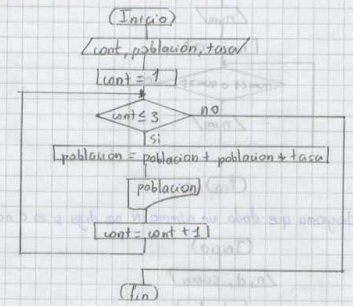
\includegraphics[width=0.6\textwidth]{Img/DF_ej14.png}
                \end{figure}

                \begin{figure}[!h]
                    \centering
                    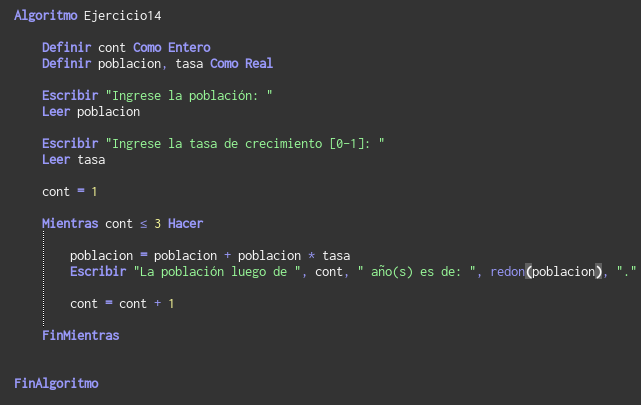
\includegraphics[width=0.7\textwidth]{Img/Cod_ej14.png}
                \end{figure}

                \begin{figure}[!h]
                    \centering
                    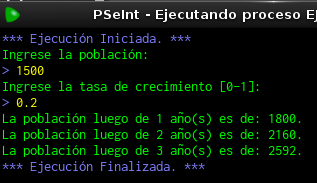
\includegraphics[width=0.5\textwidth]{Img/Ejec_ej14.png}
                \end{figure}

            % Ejercicio 15: -----------------------------------------------
            \newpage 
            \item La sucesión de Fibonacci se define de la siguiente forma: a1=1, a2=1 y an=an-1+an-2 para n>2, es decir los dos primeros son 1 y el resto cada uno es la suma de los dos anteriores, los primeros son: 1, 1, 2, 3, 5, 8, 13, 21,... Hacer un diagrama de flujo para calcular el Nésimo término de la sucesión.
                
                \begin{figure}[!h]
                    \centering
                    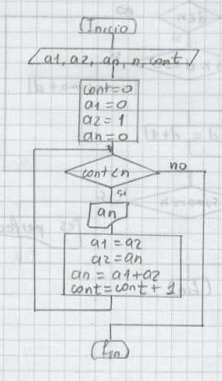
\includegraphics[width=0.4\textwidth]{Img/DF_ej15.png}
                \end{figure}

                \begin{figure}[!h]
                    \centering
                    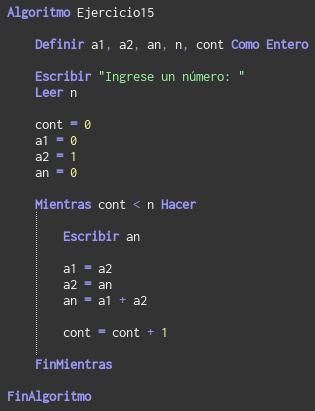
\includegraphics[width=0.4\textwidth]{Img/Cod_ej15.png}
                \end{figure}

                \begin{figure}[!h]
                    \centering
                    \includegraphics[width=0.4\textwidth]{Img/Ejec_ej15.png}
                \end{figure}

        \end{enumerate}

\end{document}